\chapter{Applications}
\label{Applications}

In this chapter, we present two applications of the discrete spherical Fourier 
transform algorithms. The first application concerns the fast summation radial
functions on the sphere -- an essential task in approximation by spherical
radial basis functions. We propose an approximative algorithm which can be
interpreted as a cutoff in 'frequency' domain with respect to the
$\Ln{2}{\twosphere}$ orthonormal basis of spherical surface functions.
The second application is the reconstruction of spherical Fourier coefficients
from scattered data on the sphere $\twosphere$ by means of iterative 
numerical algorithms. In many settings, data on the sphere is not given on
a grid corresponding to quadrature formulae which allow for the exact
computation of spherical Fourier coefficients, but on somewhat scattered sets
of nodes. The reconstruction problem is therefore formulated as a
\emph{weighted linear least squares problem} or a 
\emph{weighted optimal interpolation problem} which allows for the 
employment of iterative numerical algorithms.

\section{Fast Summation of Radial Functions on the Sphere}
\label{Applications:FastSum}
\emph{Radial basis functions} are a powerful tool in many areas of multi-dimensional 
approximation and interpolation, in particular for scattered data. Other applications
include the numerical solution of partial differential equations and artificial neural networks 
for nonparametric regression.
In radial basis function methods one approximates a function $g: \R^n
\rightarrow \R$, $n \in \N$, by a linear combination $f$ of the form
\begin{equation}
  \nonumber
  \fun{f}{\V{x}} := \sum_{l=0}^{L-1} b_{l} \fun{\phi}{\norm{\V{y}_{l}-\V{x}}} \quad 
  \paren{L \in \N,\ y_{l} \in \R^n},
\end{equation}
where $b_{l} \in \R$ for $l = 0,\ldots,L-1$, and 
$\phi: \Rp \rightarrow \R$ is a function on the positive real line. 
The functions $\set{\fun{\phi}{\norm{\V{y}-\cdot}}}_{l=0}^{L-1}$ are
denoted \emph{radial basis functions} since they depend solely on 
the distance of the argument $\V{x}$ to a fixed point $\V{y}_{l}$ measured 
by a suitable norm $\norm{\cdot}$, which is usually intended to be euclidean.
Moreover, these functions are, loosely speaking, \emph{localizing} in the sense 
that they decay rapidly outside a neighborhood of $\V{y}_{l}$.

The spherical counterpart of radial basis function are the \emph{spherical radial basis functions} 
or \emph{zonal} functions as introduced in Section 
\ref{Basics:SphericalKernels}. The norm $\norm{\V{y}_{l}-\V{x}}$ is replaced 
by the usual inner product $\V{\eta}_{l}\cdot\V{\xi}$, i.e. one
approximates a function $g: \twosphere \rightarrow \R$ by
\begin{equation}
  \label{Applications:ZonalSum}
  \fun{f}{\V{\xi}} := \sum_{l=0}^{L-1} b_{l} \fun{K}{\V{\eta}_{l}\cdot\V{\xi}} \quad 
  \paren{L \in \N,\ \V{\eta}_{l} \in \twosphere}
\end{equation}
with $b_{l} \in \R$ for $l=0,\ldots,L-1$, and 
$K: [-1,1] \rightarrow \R$ is now an $\Ln{2}{[-1,1]}$ function. 
The fact that the geodesic distance $\fun{d}{\V{\xi},\V{\eta}}$ of two points 
$\V{\xi}$ and $\V{\eta}$ on the 
sphere $\twosphere$ is $\fun{d}{\V{\eta},\V{\xi}} = 
\sqrt{2-2\V{\eta}\cdot\V{\xi}}$ justifies this choice.

An essential task is the fast evaluation of such linear combinations. More formally, 
one wants to evaluate the sum \eqref{Applications:ZonalSum}
on a set of \emph{target nodes} 
$$
  \mathcal{X} := \pset{\V{\xi}_{d} \in \twosphere}{|}{d=0,\ldots,D-1} \quad \paren{D \in \N},
$$ 
with 
$$
  \mathcal{Y} := \pset{\V{\eta}_{l} \in \twosphere}{|}{l = 0,\ldots,L-1} \quad \paren{L \in \N}
$$
being the set of so-called \emph{source nodes}.

Clearly, the construction of fast algorithms for this task depends strongly on the
choice of the function $K$, and conditions imposed on the distribution of the 
source and target nodes $\mathcal{Y}$ and $\mathcal{X}$, respectively.
If, for example, these sets of nodes are fixed for all evaluations, one might 
precompute all values $ \fun{K}{\V{\eta}_{l}\cdot\V{\xi}_{d}}$ for $l=0,\ldots,L-1$ and 
$d=0,\ldots,D-1$, just forming a weighted sum of $L$ summands for each evaluation 
at one of the $D$ target nodes $\V{\xi}_{d}$. This clearly yields an $\bigo{L D}$ algorithm.

Of course, the naive approach, i.e. evaluating \eqref{Applications:ZonalSum} for every $\V{\xi}_{d} 
\in \mathcal{X}$ leads to an $\bigo{L\:D}$ algorithm, too. 
For large $L$ and $D$ the computational effort for $\bigo{L D}$ algorithms 
becomes quickly unaffordable.

Quite effective algorithms are often derived by approximating the desired result 
up to an adjustable accuracy. In this case, the localizing property of the function $K$ 
generally has a strong impact. If the function $K$ localizes well and the source nodes 
are not, say, 'clustered' too much, one might take for the evaluation of $f$ at a single target 
node $\V{\xi}_{d}$ into consideration only those functions $\fun{K}{\V{\eta}_{l}\:\cdot}$, for
which $\V{\eta}_{l}$ lies in a certain neighborhood of $\V{\xi}_{d}$. This corresponds to 
truncating the support of the function $K$. If $K$ is already finitely supported, this even
yields exact algorithms. 
The \emph{panel clustering} method introduced in \cite{FrGlSch98} reduces the computational 
effort to evaluate \eqref{Applications:ZonalSum} based on the traditional method of dividing 
the evaluation of \eqref{Applications:ZonalSum} into near- and far-field. For every function
$\fun{K}{\V{\eta} \: \cdot}$, the near-field contribution is calculated exactly whereas the 
contribution of the far-field may be approximated coarsely due to the assumed rapid decay 
of $\fun{K}{\V{\eta} \: \cdot}$. 

Instead of the truncation idea from above, which can be interpreted as a truncation in 
'\emph{spatial}' domain, we propose a truncation in '\emph{frequency}' domain with respect 
to the $\Ln{2}{\twosphere}$ orthonormal basis  
of spherical surface functions $Y_{k}^n$. The Addition 
Theorem \ref{Basics:AdditionTheorem} provides a 
representation of the function $K$ that separates source and target nodes and 
therefore allows for the construction of fast algorithms. The connection is as 
follows: Using the representation \eqref{Basics:Kernel} from Section 
\ref{Basics:SphericalKernels}, we have
\begin{equation}
  \label{Applications:KSeries}
  \fun{K}{\V{\eta}_{l} \cdot \V{\xi}} = \sum_{k=0}^{\infty} \sum_{n=-k}^k 
  \fun{K^{\wedge}}{k}   \fun{Y_{k}^n}{\V{\xi}} \overline{\fun{Y_{k}^n}{\V{\eta}_{l}}}
\end{equation}
where we recall the symbol $K^{\wedge}$ of $K$
\[
  \fun{K^{\wedge}}{k} = 2 \pi \int_{-1}^{1} \fun{K}{x} \fun{P_{k}}{x} \dx x 
  \quad \paren{k \in \NZ}.
\]
Now, truncating at a fixed index $M \in \NZ$, i.e. setting
\begin{equation}
  \label{Applications:TruncatedSeries}
  \fun{K_{M}}{\V{\eta}_{l} \cdot \V{\xi}} := 
  \sum_{k=0}^{M} \sum_{n=-k}^k \fun{K^{\wedge}}{k} \fun{Y_{k}^n}{\V{\xi}} \overline{\fun{Y_{k}^n}{\V{\eta}_{l}}},
\end{equation}
we approximate $f$ by a function $f_{M}$ with
\begin{equation}
  \nonumber
  \begin{split}
    \fun{f_{M}}{\xi} & := \sum_{l = 0}^{L-1} b_{l} \fun{K_{M}}{\V{\eta}_{l} \cdot \V{\xi}} \\
                 &       = \sum_{l = 0}^{L-1} b_{l} \sum_{k=0}^{M} \sum_{n=-k}^k \fun{K^{\wedge}}{k}
                           \fun{Y_{k}^n}{\V{\xi}} \overline{\fun{Y_{k}^n}{\V{\eta}_{l}}} \\
                 &       = \sum_{k=0}^{M} \sum_{n=-k}^k \paren{\sum_{l = 0}^{L-1} b_{l}
                           \overline{\fun{Y_{k}^n}{\V{\eta}_{l}}}} \fun{K^{\wedge}}{k} \fun{Y_{k}^n}{\V{\xi}}.
  \end{split}                           
\end{equation}
The sums
\begin{equation}
\label{Applications:AdjointNDSFT}
  \tilde{b}_{k}^n := \sum_{l = 0}^{L-1} b_{l} \overline{\fun{Y_{k}^n}{\V{\eta}_{l}}} \quad \paren{(k,n) \in \mathcal{I}^M}
\end{equation}
in brackets can be evaluated by an adjoint NFSFT (Algorithm 
\ref{NFSFT:Algorithm:adjointNFSFT}) and we arrive at
\[
  \fun{f_{M}}{\xi} = \sum_{k=0}^{M} \sum_{n=-k}^k \tilde{b}_{k}^n \fun{K^{\wedge}}{k}
                     \fun{Y_{k}^n}{\V{\xi}} = \sum_{k=0}^{M} \sum_{n=-k}^k a_{k}^n
                     \fun{Y_{k}^n}{\V{\xi}},
\]
where we let $a_{k}^n := \tilde{b}_{k}^n \fun{K^{\wedge}}{k}$. Finally, the evaluation of
\begin{equation}
\label{Applications:NDSFT}
  \fun{f_{M}}{\V{\xi}} = \sum_{k=0}^{M} \sum_{n=-k}^k a_{k}^n \fun{Y_{k}^n}{\V{\xi}}
\end{equation}
on the set of target nodes $\mathcal{X}$ can be carried out by a NFSFT 
(Algorithm \ref{NFSFT:Algorithm:NFSFT}). The presented NFSFT algorithms have arithmetic complexity 
$\bigo{M^3 \log M + \fun{\log}{1/\varepsilon}L}$ and 
$\bigo{M^3 \log M + \fun{\log}{1/\varepsilon}D}$, respectively. The intermediate 
step consists in computing the coefficients $a_{k}^n$ by $\bigo{M^2}$ multiplications
with the symbol $\fun{K^{\wedge}}{k}$. Since $M$ is fixed, we have in total an
$\bigo{L + D}$ algorithm for the evaluation of $f_{M}$ on $\mathcal{X}$. In particular, the
performance does not depend on the distribution of the source and target nodes, 
$\V{\eta}_{l}$ and $\V{\xi}_{d}$. We summarize this procedure in Algorithm 
\ref{Applications:Algorithm:FastSummation}.

\begin{remark}
  The proposed algorithm is approximative in multiple ways: First, the systematic 
  error introduced by truncating the series \eqref{Applications:KSeries} at the 
  index $M$ limits the 
  achievable accuracy. Moreover, the NFSFT algorithm and its adjoint 
  are approximative themselves. First, the FLFT part is limited by the choice of the
  threshold during precomputation. Second, the invocation of the NFFT and adjoint 
  NFFT algorithms introduces an error, since these algorithms are by definition yet
  approximative. In total, one has to adjust the corresponding parameters accordingly 
  to yield an accurate result.
  However, replacing the NFSFT and adjoint NFSFT by its direct versions called NDSFT and 
  adjoint NDSFT still yields an $\bigo{L + D}$. Under the assumption that these are 
  stable, $M$ remains the only accuracy-limiting parameter.
\end{remark}

\begin{remark}
  Algorithm \ref{Applications:Algorithm:FastSummation} also admits complex 
  coefficients $b_{l} \in \C$. This gives rise to generally complex valued 
  linear combinations $f$. Moreover, we could also permit complex-valued 
  symbol coefficients $\fun{K^{\wedge}}{k,n} \in \C$ that even depend on $n$. 
\end{remark}

\begin{remark}
	The summation algorithm can be expressed in matrix-vector notation. This reads
	\[
	  \V{f}_{\mathcal{X}} = \V{Y}_{\mathcal{X}} \: \V{W} \:
	  \V{Y}_{\mathcal{Y}}^{\h} \: \V{b}
	\]
	with
	\begin{align}
	  \nonumber
	  \V{f}_{\mathcal{X}} & := \paren{\fun{f_{M}}{\V{\xi}_{d}}}_{d=0}^{D-1} \in \R^D,\\
	  \nonumber
	  \V{Y}_{\mathcal{X}} & := \paren{\fun{Y_k^n}{\V{\xi}_{d}}}_{d=0,\ldots,D-1; 
	  \paren{k,n} \in \mathcal{I}^M} \in \C^{D \times \paren{M+1}^2}, \\
	  \nonumber
	  \V{W} & := \fun{\diag}{\V{w}},\ \V{w} := \paren{w_{k}^n}_{\paren{k,n} \in 
	  \mathcal{I}^M} \in \R^{(M+1)^2},\ w_{k}^n := \fun{K^{\wedge}}{k}, \\
	  \nonumber
	  \V{Y}_{\mathcal{Y}} & := \paren{\fun{Y_k^n}{\V{\eta}_{l}}}_{l=0,\ldots,L-1;
	  \paren{k,n} \in \mathcal{I}^M} \in \C^{L \times \paren{M+1}^2}.
	\end{align}
\end{remark}

\begin{algorithm}[tb]
  \caption{Fast Summation of Spherical Radial Functions}
  \label{Applications:Algorithm:FastSummation}    
  \begin{algorithmic}
    \STATE  Input:  $L \in \N$, $\paren{b_{l}}_{l=0}^{L-1}$, 
    $\paren{\V{\eta}_{l}}_{l=0}^{L-1}$, $D \in \N$, 
    $\paren{\V{\xi}_{d}}_{d=0}^{D-1}$, $M \in \NZ, 
    \paren{\fun{K^{\wedge}}{k}}_{k=0}^M$
    \STATE
    \STATE Compute $\paren{\tilde{b}_{k}^n}_{\paren{k,n} \in \mathcal{I}^M}$ 
    by a fast adjoint NFSFT
    \STATE 
    \FOR {$k=0,\ldots,M$} 
      \FOR {$n=-k,\ldots,k$} 
        \STATE $a_{k}^n := \tilde{b}_{k}^n \fun{K^{\wedge}}{k}$
      \ENDFOR
    \ENDFOR
    \STATE
    \STATE Compute $\paren{\fun{f}{\V{\xi}_{d}}}_{d=0}^{D-1}$ by a fast NFSFT
    \STATE
    \STATE Output: $\paren{\fun{f}{\V{\xi}_{d}}}_{d=0}^{D-1}$
\end{algorithmic}
\end{algorithm}

\subsection{Error Estimates}

\begin{lemma}\label{lemma:error}
  The proposed approximation $f_{M}$ obeys the uniform error estimate
  \begin{equation}
    \label{Applications:UniformErrorBound}
    \left\|f - f_{M}\right\|_{\infty} \le \left\|\V{b}\right\|_1 \sum_{k>M}
    \frac{2k+1}{4\pi} \abs{\fun{K^{\wedge}}{k}}.
  \end{equation}
\end{lemma}
\begin{proof}
  We obtain immediately
  \begin{align*}
    \left\|f - f_{M}\right\|_{\infty} 
    & = \max_{\V{\xi} \in \twosphere} 
        \left|\sum_{l=0}^{L-1} b_{l} \sum_{k>M} \frac{2k+1}{4\pi} \fun{K^{\wedge}}{k} 
        \fun{P_{k}}{\V{\eta}_{l} \cdot \V{\xi}}\right| \\
    & \le \sum_{l=0}^{L-1} \left| b_{l} \right| \max_{\V{\xi} \in \twosphere} 
      \left| \sum_{k>M} \frac{2k+1}{4\pi} \fun{K^{\wedge}}{k} 
      \fun{P_{k}}{\V{\eta}_{l} \cdot \V{\xi}} \right| \\
    & \le \left\|\V{b}\right\|_1 \sum_{k>M} \frac{2k+1}{4\pi} \abs{\fun{K^{\wedge}}{k}},
  \end{align*}
  where we have used $\left|\fun{P_{k}}{x}\right| \le 1$ for $x \in [-1,1]$. 
\end{proof}

For the Poisson kernel \eqref{PoissonKernel} and the singularity kernel
\eqref{SingularityKernel}, we have thereby the following lemma.

\begin{lemma}${}^{}$\\[-3.5ex]
 \begin{enumerate}
   \item 
Using the Poisson kernel with $Q_h$ in our summation algorithm yields a relative 
error of
     \begin{equation}
       \label{error:poisson}
       \frac{\left\|f - f_{M}\right\|_{\infty}}{\left\|\V{b}\right\|_1} \le
       \frac{h^{M+1}}{4\pi}
       \left(\frac{2M+1}{1-h}+\frac{2}{\left(1-h\right)^2}\right)\quad \paren{h \in (0,1)}.
     \end{equation}
     \item 
Using the singularity kernel with $S_h$ in our summation algorithm yields 
a relative error of
       \begin{equation}
         \label{error:singular}
         \frac{\left\|f - f_{M}\right\|_{\infty}}{\left\|\V{b}\right\|_1} \le
         \frac{h^{M+1}}{4\pi} \left(\frac{2M+1}{2\left(1-h\right)}+
           \frac{4M}{\left(1-h\right)^2}+
         \frac{4}{\left(1-h\right)^3}\right)\quad \paren{h \in (0,1)}.
       \end{equation}
 \end{enumerate}
\end{lemma}
\begin{proof}
The symbols are given by $\fun{Q_{h}^{\wedge}}{k}=h^k$ and
$\fun{S_{h}^{\wedge}}{k}=\frac{2}{2k+1}h^k$, respectively.
Using Lemma \ref{lemma:error} yields the assertions.
\end{proof}
Thus, the error decays exponentially with increasing $M$.
The locally supported kernels $L_{h,\lambda}$ defined in Section 
\ref{Basics:SphericalKernels} also obey the uniform error bound
\eqref{Applications:UniformErrorBound}. But in contrast to the Poisson kernel 
and the Singularity kernel we obtain only a polynomial error decay in $M$.
\begin{lemma}
  For the locally supported kernels $L_{h,\lambda}$ holds:
  \begin{enumerate}
  \item We obtain for $\lambda \in \NZ$ and $k>\lambda+1$ the decay rate
    \[
    \left|\fun{L_{h,\lambda}^{\wedge}}{k}\right| \le
    \frac{2\sqrt{2}}{\paren{2k+1}\sqrt{\pi}}
    \frac{\paren{\lambda+1}^2}{\paren{1-h}^{2\lambda+1}\sqrt[4]{1-|h|}}
    \frac{1}{\paren{k-\lambda}^{\lambda+\frac{1}{2}}}\,. 
    \]
  \item Thus, the relative error of our summation algorithm with this kernel
  $K=L_{h,\lambda}$ is bounded for $\lambda \in \N$ and $M>\lambda$ by
  \begin{equation}
    \label{error:Lh}
    \frac{\left\|f - f_{M}\right\|_{\infty}}{\left\|\V{b}\right\|_1} \le
    \frac{1}{\pi\sqrt{2\pi}}
    \frac{\paren{\lambda+1}^2}{\lambda-\frac{1}{2}}
    \frac{1}{\paren{1-h}^{2\lambda+1}\sqrt[4]{1-|h|}}
    \frac{1}{\paren{M-\lambda}^{\lambda-\frac{1}{2}}}\,.
  \end{equation}
  \end{enumerate}
\end{lemma}

\begin{proof}${}^{}$\\[-3.5ex]
  \begin{enumerate}
  \item For $\lambda=0$, we have
    \begin{equation*}
      \left|\fun{L_{h,\lambda}^{\wedge}}{k}\right| 
      = \abs{2\pi \int_{h}^1 \frac{\lambda+1}{2\pi\paren{1-h}^{\lambda+1}} 
        \paren{x-h}^{\lambda} \fun{P_{k}}{x} \: \dx x} 
      \le \frac{\lambda+1}{(1-h)^{\lambda+1}}\abs{\int_{h}^1 \fun{P_{k}}{x} \: \dx x}.
    \end{equation*}
    Using \eqref{three2} and $\left|\fun{P_{k}}{\cos\vartheta}\right|
    \le \sqrt{\frac{2}{\pi k \sin\vartheta}}$ for $\vartheta \in (0,\pi)$, we obtain
    \begin{align*}
      \abs{\int_{h}^1 \fun{P_{k}}{x} \: \dx x}
      %& = \frac{1}{2k+1}
      %    \abs{\int_{h}^1 \fun{P_{k+1}'}{x} - \fun{P_{k-1}'}{x} \: \dx x}\\
      & = \frac{1}{2k+1}
          \abs{\fun{P_{k-1}}{h} - \fun{P_{k+1}}{h}}\\
      & \le \frac{1}{2k+1} \sqrt{\frac{2}{\pi \sin\arccos h}} \paren{\frac{1}{\sqrt{k-1}} + \frac{1}{\sqrt{k+1}}},
    \end{align*}
    and with $\sin\arccos h = \sqrt{1-h^2} \ge \sqrt{1-|h|}$ and
    $\frac{1}{\sqrt{k-1}} + \frac{1}{\sqrt{k+1}} \le
    \frac{2k+1}{k\sqrt{k}}$ finally
    \begin{equation}
      \label{SmallLambda}
      \left|\fun{L_{h,0}^{\wedge}}{k}\right| \le 
      \frac{\sqrt{2}}{\sqrt{\pi}}\frac{\lambda+1}{(1-h)^{\lambda+1}\sqrt[4]{1-|h|}}
      \frac{1}{k\sqrt{k}}.
    \end{equation}
%    \frac{1}{1-h}
%    \left|\int_{h}^{1} \fun{P_{k}}{x} \dx x\right| \le
%    \frac{\sqrt{2}}{\left(2k+1\right)\left(1-h\right)\sqrt{\pi}\sqrt[4]{1-h^2}}
%    \left(\frac{1}{\sqrt{k-1}}+\frac{1}{\sqrt{k+1}}\right)\,.
    Furthermore, for $\lambda \in \N$, we obtain by applying \eqref{three2} that
    \begin{equation*}
      \left|\fun{L_{h,\lambda}^{\wedge}}{k}\right| 
      %&\le&
      %\frac{\lambda+1}{\lambda\left(1-h\right)\left(2k+1\right)}
      %\left|\fun{L_{h,\lambda-1}^{\wedge}}{k-1}-
      %  \fun{L_{h,\lambda-1}^{\wedge}}{k+1}\right|\\ &\le&
      \le \frac{2}{2k+1} \frac{\lambda+1}{\lambda\left(1-h\right)}
      \max\limits_{|k-k'|\le 1}
      \left|\fun{L_{h,\lambda-1}^{\wedge}}{k'}\right|.
    \end{equation*}
    Iterate this argument and estimate $\frac{2}{2k'+1}\le
    \frac{1}{k-\lambda}$ yields
    \begin{align*}
      \left|\fun{L_{h,\lambda}^{\wedge}}{k}\right|
      & \le \frac{2}{2k+1} \frac{\lambda+1}{\paren{1-h}^{\lambda}}
        \frac{1}{\paren{k-\lambda}^{\lambda-1}} 
        \max_{|k-k'| \le \lambda} 
        \abs{\fun{L_{h,0}^{\wedge}}{k'}}.
    \end{align*}
    We finally use \eqref{SmallLambda} for $k'=k-\lambda$ to obtain the
    assertion.
  \item We combine 1. with Lemma \ref{lemma:error}. 
  \end{enumerate}
\end{proof}

As the last example, we consider the spherical Gaussian kernel $G_{\sigma}$. 

\begin{lemma}
  The Gaussian-kernel $G_{\sigma}$ obeys the error bound
  \begin{equation}
    \label{error:G}
    \frac{\left\|f - f_{M}\right\|_{\infty}}{\left\|\V{b}\right\|_1} \le
    \frac{\sqrt{\pi\sigma}\left(\e^{\sigma}-1\right) \sigma^{M-\frac{1}{2}}}{\fun{\Gamma}{M
    +\frac{1}{2}}}.
  \end{equation} 
\end{lemma}
\begin{proof}
  Using $\fun{G_{\sigma}^{\wedge}}{k} = \sigma^{-\frac{1}{2}} \e^{-\sigma}
  \pi^{\frac{3}{2}} \fun{I_{k+\frac{1}{2}}}{\sigma}$ and
  \begin{eqnarray*}
    \frac{2k+1}{4\pi} \abs{\fun{G_{\sigma}^{\wedge}}{k}}
    &=&
    \frac{\e^{-2\sigma}
    \left(k+\frac{1}{2}\right)\sigma^k}{\fun{\Gamma}{k+1}} \int_{-1}^{1}
    \e^{2\sigma x} \left(1-x^2\right)^k \dx x\\
    &\le&
    \frac{\left(k+\frac{1}{2}\right)\sigma^k}{\fun{\Gamma}{k+1}}
    \int_{-1}^{1} \left(1-x^2\right)^k \dx x\\
    &=&
    \frac{\sqrt{\pi}\sigma^k}{\fun{\Gamma}{k+\frac{1}{2}}}
  \end{eqnarray*}
  in conjunction with
  \begin{equation*}
    \sum_{k>M} \frac{\sqrt{\pi}\sigma^k}{\fun{\Gamma}{k+\frac{1}{2}}}\\
    =
    \frac{\sqrt{\pi\sigma}\e^{\sigma}}{\fun{\Gamma}{M+\frac{1}{2}}} 
    \int_{0}^{\sigma} t^{M-\frac{1}{2}} \e^{-t} \dx t\\
    \le
    \frac{\sqrt{\pi\sigma}\left(\e^{\sigma}-1\right) \sigma^{M-\frac{1}{2}}}{\fun{\Gamma}{M
    +\frac{1}{2}}}
  \end{equation*}
  yields the assertion.
\end{proof}

\subsection{Numerical Tests}

\begin{figure}[tb]
  \centering
  \subfigure[The Poisson kernel $Q_{h}$ for $h = 0.8$.]
  { \label{SubFigurePoisson}
    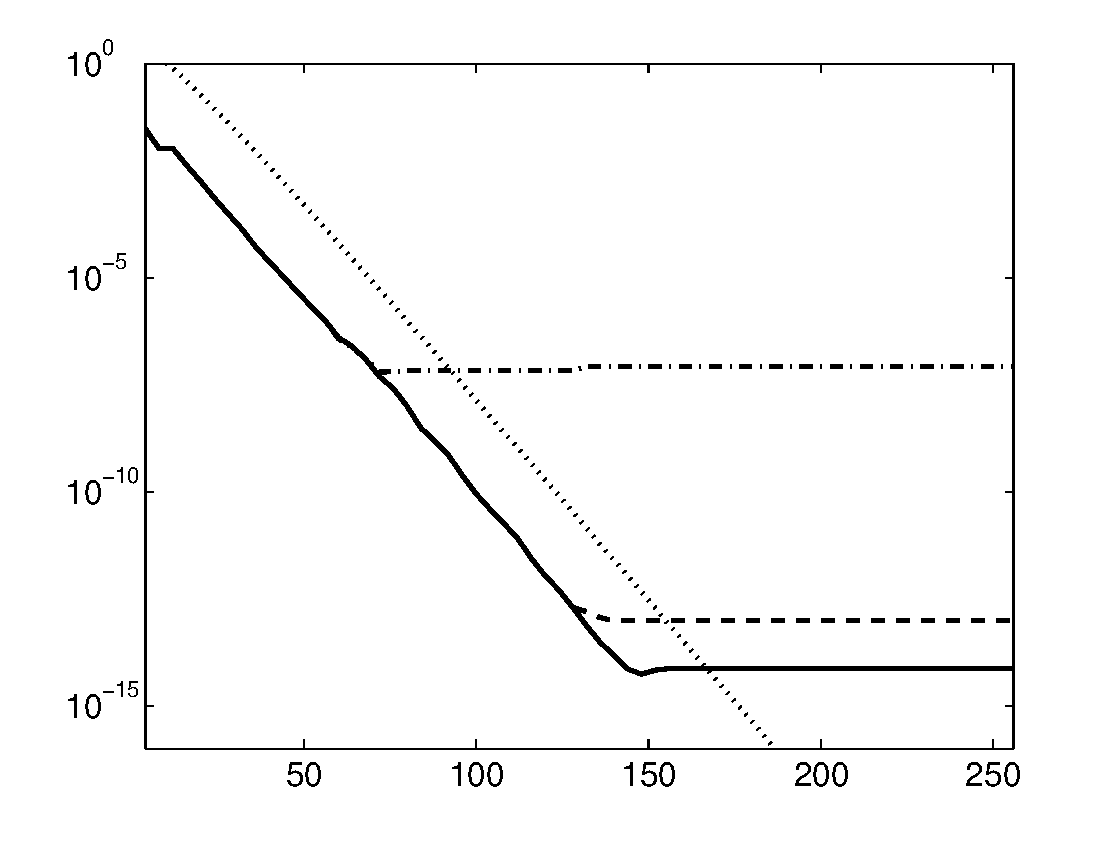
\includegraphics[width=0.45\textwidth]{images/poisson_test}}\hfill
  \subfigure[The Singularity kernel $S_{h}$ for $h = 0.8$.]
  {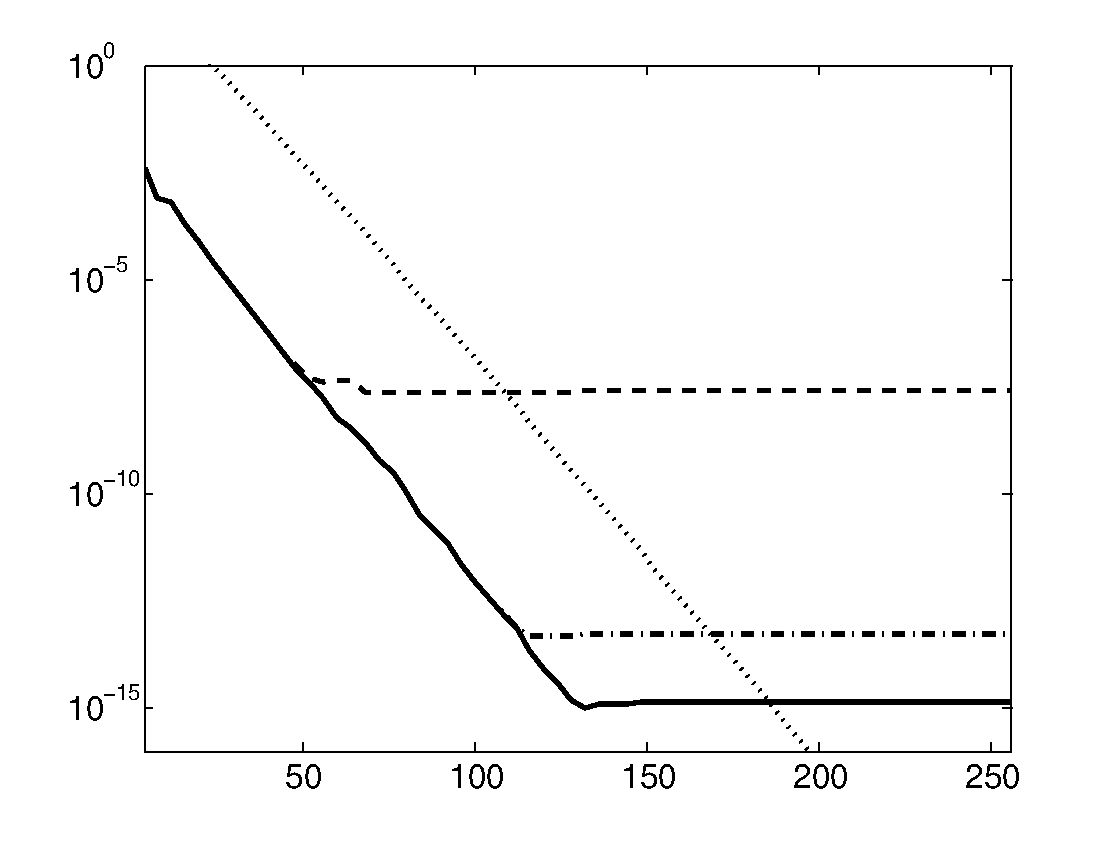
\includegraphics[width=0.45\textwidth]{images/singularity_test}}\\
  \caption{The error $E_{\infty}$ for $k = 4,8,\ldots,256$ and $L = D = 1000$: 
  Fast summation with NDSFT (solid), fast summation with NFSFT, 
  NFFT cut-off parameter $m = 3$ and FLFT threshold $t = 10^6$ (dash-dot), 
  fast summation with NFSFT, NFFT cut-off 
  parameter $m = 6$ and FLFT threshold $t = 10^6$ (dashed), error estimate for 
  $E_{\infty}$ (dotted).}
  \label{fig:error}
\end{figure}

We present numerical examples in order to demonstrate the performance of
our approach. All algorithms were implemented in C and tested on an 
AMD Athlon\texttrademark XP 2700+ with 2GB main memory, SuSe-Linux 
(kernel 2.4.20-4GB-athlon, gcc 3.3) using double precision arithmetic. 
Moreover, we have used the libraries FFTW 3.0.1 \cite{fftw}, NFFT 2
\cite{kupo02C} and a custom NFSFT library which will be part of the next 
major release of the NFFT library. Throughout our experiments we have 
applied the NFFT package \cite{kupo02C} with precomputed Kaiser--Bessel 
functions and an oversampling factor $\rho=2$.

In our tests we have always chosen uniformely distributed pseudo-random 
source and target nodes 
$\paren{\vartheta,\varphi} \in [0,\pi] \times [-\pi,\pi]$ and 
coefficients $b_l$ from $\left[-\frac{1}{2},\frac{1}{2}\right]$.

\begin{figure}[tb]
  \centering
  \subfigure[The locally supported kernel $L_{h,\lambda}$ for $h=0.3$, $\lambda = 7$. 
  The error estimate was fitted using $C_{\lambda} = 100$. For $C_{\lambda} = 50$ 
  it virtually coincides with the numerical result.]
  {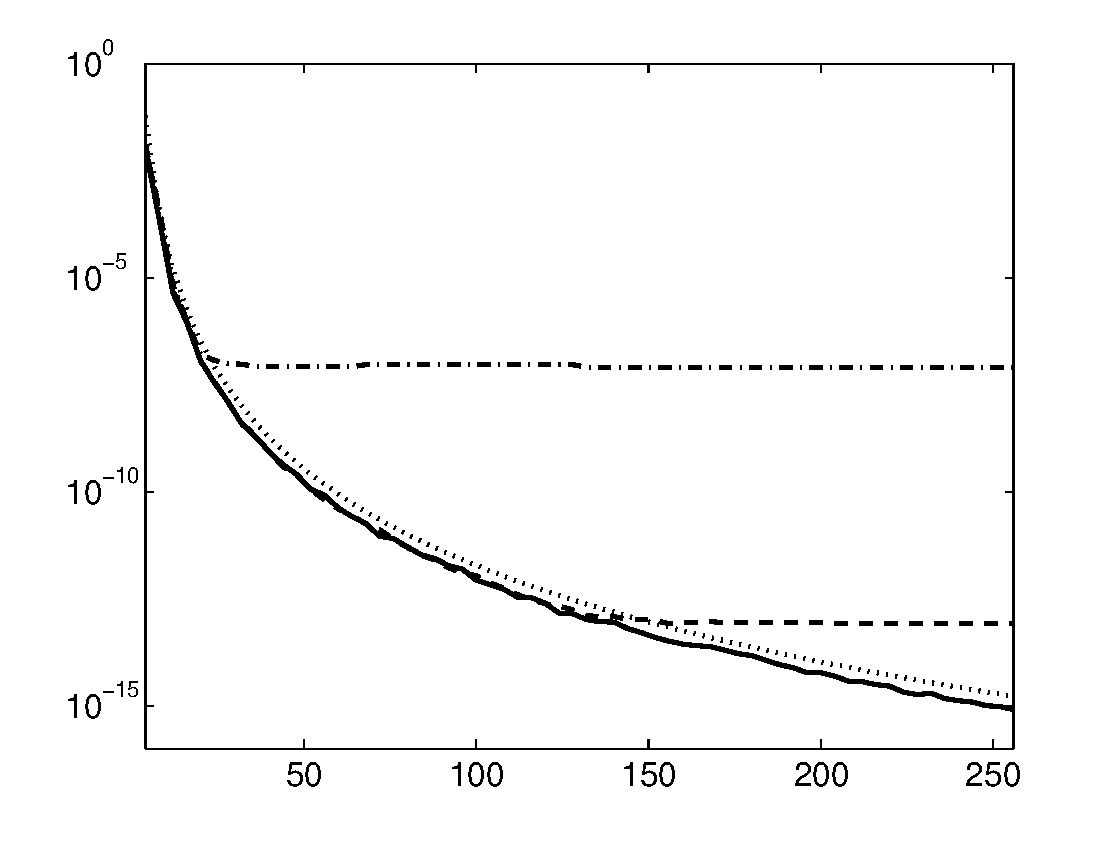
\includegraphics[width=0.45\textwidth]{images/locsupp_test}}\hfill
  \subfigure[The Gaussian kernel $G_{\sigma}$ for $\sigma=200$. The corresponding
  error estimate from \eqref{error:G} does not provide a useful error bound.]
  {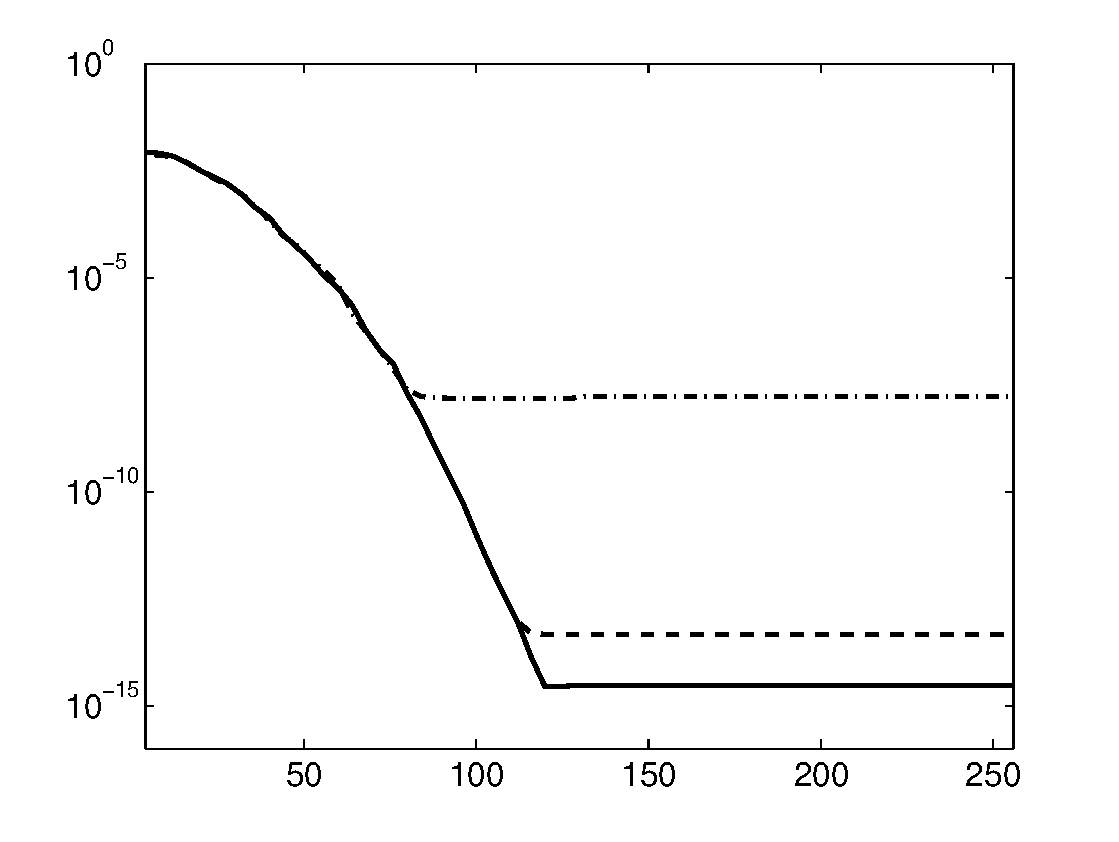
\includegraphics[width=0.45\textwidth]{images/gaussian_test}}
  \caption{The error $E_{\infty}$ for $k = 4,8,\ldots,256$ and $L = D = 1000$: 
  Fast summation with NDSFT (solid), fast summation with NFSFT, 
  NFFT cut-off parameter $m = 3$ and FLFT threshold $t = 10^6$ (dash-dot), 
  fast summation with NFSFT, NFFT cut-off parameter $m = 6$ and FLFT threshold 
  $t = 10^6$ (dashed), error estimate for $E_{\infty}$ (dotted).}
  \label{fig:error2}
\end{figure}

First, we examine the systematic error due to our approximation 
\eqref{Applications:TruncatedSeries} and the use of the 
approximative NFSFT algorithm. Figures \ref{fig:error} and
\ref{fig:error2} present
the error
\[
  E_{\infty}:=
  \frac{\left\|\V{f}-\V{f}_M\right\|_{\infty}}{\left\|\V{b}\right\|_{1}}
  \quad \approx \quad \frac{\left\|f-f_M\right\|_{\infty}}{\left\|\V{b}\right\|_{1}}
\]
for the considered kernels as a function of the parameter $M$.
These results confirm the error estimates \eqref{error:poisson},
\eqref{error:singular} and \eqref{error:Lh}. 
In Figure \ref{hTest},
we used in addition a second value $h=0.7$ for the locally supported 
kernel $L_{h,\lambda}$ in order to emphasize that the error 
bound is mainly dominated by the terms that depend on $\lambda$.

In order to 
demonstrate and isolate the specific influence of the threshold 
for the FLFT algorithm, we applied the fast summation algorithm 
to the Poisson kernel with the same parameters as in Figure 
\ref{SubFigurePoisson}, but with internally deactivated NFFT 
algorithm. Instead, we used the direct exact NDFT algorithm to 
evaluate the corresponding part. The result in Figure \ref{tTest}
shows that, 
apparently, from a certain bandwidth $M$ on, a high threshold 
limits the accuracy of the
whole algorithm due to instable multiplication steps in the
FLFT algorithm. The situation even gets worse for increasing
$M$ as more and more instable steps are introduced into the 
cascade summation procedure.

\begin{figure}[tb]
  \centering
  \subfigure[The locally supported kernel $L_{h,\lambda}$ for $\lambda = 7$, and $h=0.3$ (solid),
  and $h=0.7$ (dashed). Computations were performed with the NDSFT algorithm. 
  The error estimate (dotted) for $E_{\infty}$ was fitted using 
  $C_{\lambda} = 100$.]
  {
    \label{hTest}
    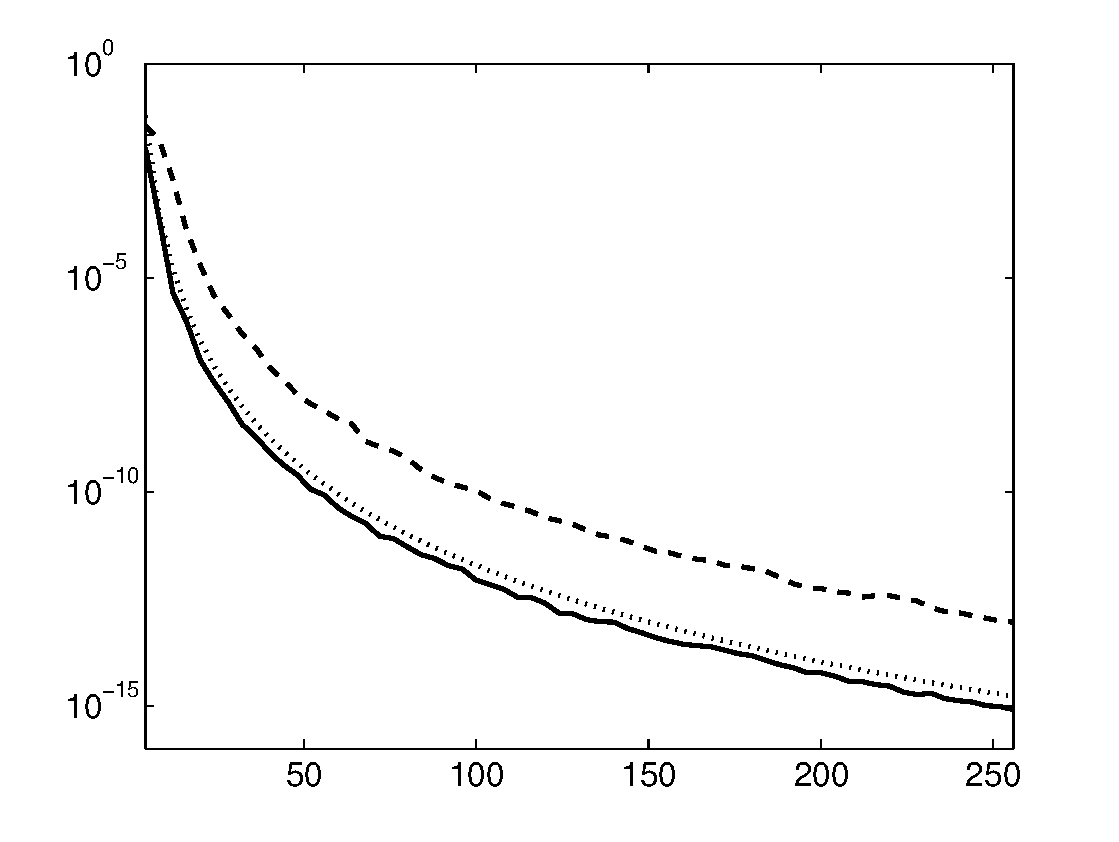
\includegraphics[width=0.45\textwidth]{images/locsup_h_test}}\hfill
  \subfigure[The Poisson kernel $Q_{h}$ for $h = 0.8$: Fast summation with 
  NFSFT, but internal use of NDFT for FLFT thresholds 
  $t=10^6$ (solid), $t=10^9$ (dashed), $t=10^9$ (dash-dot). 
  The threshold limits the accuracy of the FLFT transformation.]
  {
    \label{tTest}
  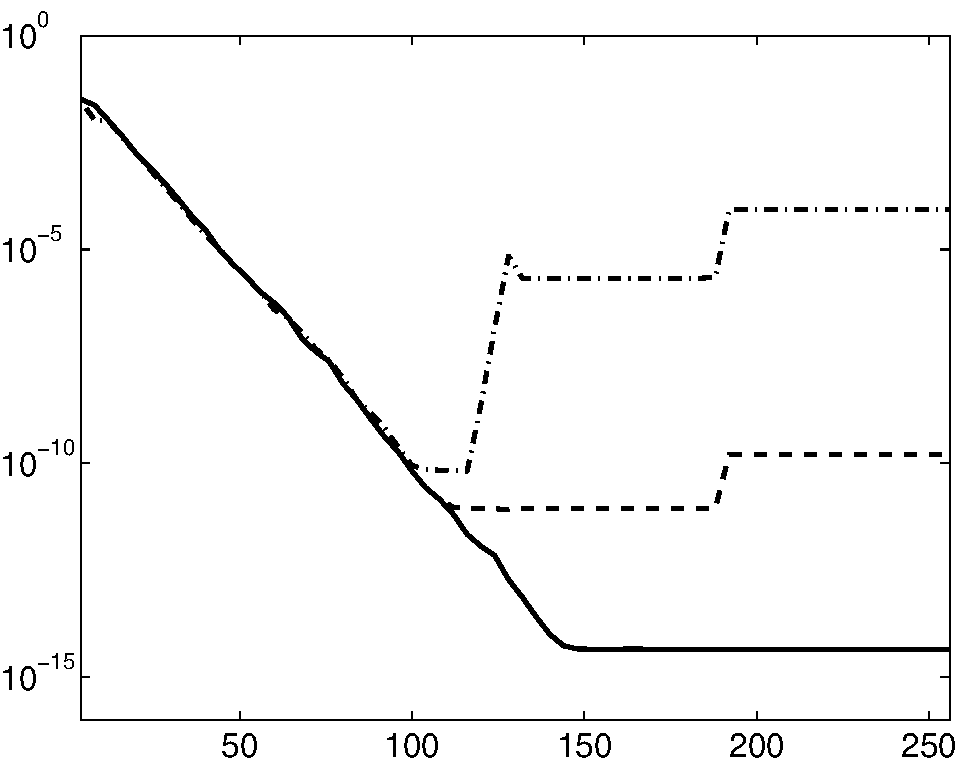
\includegraphics[width=0.45\textwidth]{images/threshold_test}}
  \caption{The error $E_{\infty}$ for $k = 4,8,\ldots,256$ and $L = D = 1000$.}
  \label{Figure:PoissonTest}
\end{figure}

Finally, we compare the computation time of the straightforward summation 
(direct algorithm), the straightforward summation with precomputed values 
$\fun{K}{\V{\eta}_{l} \cdot \V{\xi}_{d}}$, the fast summation algorithm (FS) 
with NDSFT, and the fast summation algorithm with NFSFT for increasing $L=D$.
The CPU time required by the four algorithms is shown in Table 
\ref{tab:TimeSpace}. As expected, the $\bigo{D + L}$ summation algorithms outperform the
straightforward algorithms for larger $L=D$. In addition, the NFSFT variant is 
considerably faster.

\begin{table}[ht]
  \begin{center}
    \begin{tabular}{r|r|r|r|r|r}
        $L = D$ & direct alg. & w/precomp. & FS, NDSFT & FS, NFSFT & error $E_{\infty}$\\\hline
           $2^6$ & \verb#1.0E-05# & \verb#8.0E-05# & \verb#1.1E-01# & \verb#6.2E-01# & \verb#7.7E-14# \\
           $2^7$ & \verb#6.0E-05# & \verb#3.8E-04# & \verb#2.2E-01# & \verb#6.2E-01# & \verb#6.5E-14# \\
           $2^8$ & \verb#2.5E-04# & \verb#1.4E-03# & \verb#4.5E-01# & \verb#6.2E-01# & \verb#4.1E-14# \\
           $2^9$ & \verb#1.0E-03# & \verb#5.3E-03# & \verb#8.9E-01# & \verb#6.3E-01# & \verb#2.8E-14# \\
        $2^{10}$ & \verb#4.0E-02# & \verb#2.1E-02# & \verb#1.8E+00# & \verb#6.5E-01# & \verb#3.6E-14# \\
        $2^{11}$ & \verb#1.6E+00# & \verb#8.3E-02# & \verb#3.6E+00# & \verb#6.6E-01# & \verb#1.8E-14# \\
        $2^{12}$ & \verb#6.4E+00# & \verb#3.5E-01# & \verb#7.1E+00# & \verb#7.2E-01# & \verb#1.3E-14# \\
        $2^{13}$ & \verb#2.6E+01# & \verb#1.4E+00# & \verb#1.4E+01# & \verb#8.2E-01# & \verb#6.7E-15# \\
        $2^{14}$ & \verb#1.0E+02# & \verb#-#       & \verb#2.8E+01# & \verb#1.0E+00# & \verb#5.5E-15# \\
        $2^{15}$ & \verb#4.1E+02# & \verb#-#       & \verb#5.7E+01# & \verb#1.5E+00# & \verb#4.0E-15# \\
        $2^{16}$ & \verb#1.6E+03# & \verb#-#       & \verb#1.1E+02# & \verb#2.3E+00# & \verb#2.9E-15# \\
        $2^{17}$ & \verb#6.6E+03# & \verb#-#       & \verb#2.3E+02# & \verb#4.0E+00# & \verb#2.4E-15# \\
        $2^{18}$ & \verb#2.6E+04# & \verb#-#       & \verb#4.6E+02# & \verb#7.5E+00# & \verb#1.9E-15# \\
        $2^{19}$ & \verb#-#       & \verb#-#       & \verb#9.1E+02# & \verb#1.4E+01# & \verb#-# \\
        $2^{20}$ & \verb#-#       & \verb#-#       & \verb#1.8E+03# & \verb#2.8E+01# & \verb#-# \\
        $2^{21}$ & \verb#-#       & \verb#-#       & \verb#3.6E+03# & \verb#5.5E+01# & \verb#-# \\
    \end{tabular}
  \end{center}
  \caption{CPU-Time in seconds and the error $E_{\infty}$ for the fast summation algorithm. We used 
    the Gaussian kernel $G_{\sigma}$ with $\sigma=200$ and bandwidth $M = 128$. Note that the timings 
    up to $L=D=2^{11}$ were
    averaged to compensate for measurement inaccuracies due to small computation times. The
    times/errors '$-$' are not displayed due to the large response time or memory limitations.}
  \label{tab:TimeSpace}
\end{table}


\section{Iterative Fourier Reconstruction}

In Section \ref{NFSFT:iDSFT}, we derived
inversion formulae based on quadrature rules and related to special spherical 
grids like $\mathcal{X^{\gl}}$ or $\mathcal{X^{\cc}}$. They allow for the 
reconstruction of spherical Fourier coefficients from the corresponding
function samples on these grids.
In this section we will address the problem of computing Fourier coefficients from
scattered data on the sphere $\twosphere$. To be more precise, we want to compute 
Fourier coefficients $\paren{a_{k}^n}_{(k,n) \in \mathcal{I}^M}$ up to a fixed 
bandwidth $M \in \NZ$ from function samples $\paren{f_{d}}_{d=0}^D$ given on an
arbitrary sampling set $\mathcal{X}$ with $D \in \N$ nodes, i.e. a 'solution' to
\begin{equation}
  \label{Applications:Problem}
  \V{Y} \V{a} \approx \V{f},
\end{equation}
where it remains to be specified what an admissible 'solution' of 
\eqref{Applications:Problem} is.
The matrix $\V{Y}$ in \eqref{Applications:Problem} is generally 
neither hermitian nor even square. Depending on the dimensions of $\V{Y}$, i.e.
whether the system \eqref{Applications:Problem} is \emph{over-} or 
\emph{underdetermined}, we consider two problems: the 
\emph{weighted linear least squares problem} and the
\emph{weighted optimal interpolation problem}.

\subsection{The Weighted Linear Least Squares Problem}
  For a comparatively low bandwidth, i.e. $(M+1)^2 \le D$, the matrix $\V{Y}$ 
  has more rows than columns and the system \eqref{Applications:Problem} is 
  overdetermined. We therefore consider the following problem:
  \begin{definition}
    Let $M \in \NZ$, $D \in \N$, $\mathcal{X}=\paren{\V{\xi}_{d}}_{d=0}^{D-1} \subset \twosphere$, 
    $\V{f}=\paren{f_{d}}_{d=0}^{D-1} \in \C^{D}$ and 
    \[
      \V{W} := \fun{\diag}{\paren{w_{d}}_{d=0}^{D-1}},\quad w_{d} \in \Rp \ \paren{d=0,\ldots,D-1}
    \]
    be given with $(M+1)^2 \le D$. The problem of finding a vector $\V{a}=\paren{a_{k}^n}_{(k,n) 
    \in \mathcal{I}^M}$ of spherical Fourier coefficients with
    \begin{equation}
      \label{Applications:Min}
      \norm{\V{f} - \V{Y}\:\V{a}}_{\V{W}}^2 = \text{min!}
    \end{equation}
    is called a \emph{weighted linear least squares problem}.
  \end{definition}
  The idea to use a weighted euclidean norm $\norm{\cdot}_{\V{W}}$ is to compensate for variations in
  the density distribution of the nodes $\V{\xi}_{d}$ in different regions on the sphere 
  $\twosphere$. One might reasonably wish to weight the influence of nodes in sparsely 
  represented regions more than in dense regions. The following lemma shows that a solution to
  \eqref{Applications:Min} can be obtained as a solution of a
  \emph{weighted normal equation of the first kind}.
  \begin{lemma}
    Problem \eqref{Applications:Min} is equivalent to the 
    \emph{weighted normal equation of the first kind}
    \begin{equation}
      \label{Applications:NormalEquation1}
      \V{Y}^{\h} \: \V{W} \: \V{Y} \V{a} = \V{Y}^{\h} \: \V{W} \: \V{f}.
    \end{equation}
    Moreover, \eqref{Applications:NormalEquation1} has at least one solution.
    The solution is unique if the matrix $\V{Y}$ has full rank.
  \end{lemma}
  \begin{proof}
    The expression 
    \[
      \norm{\V{f} - \V{Y}\:\V{a}}_{\V{W}}^2 = 
      \norm{\V{W}^{1/2}\paren{\V{f} - \V{Y}\:\V{a}}}_{2}^2 = 
      \norm{\V{W}^{1/2}\:\V{f} - \V{W}^{1/2}\:\V{Y}\:\V{a}}_{2}^2 = \text{min}
    \]  
    is equivalent to
    $\V{r} \perp \fun{\mathcal{R}}{\V{W}^{1/2}\:\V{Y}}$ with $\V{r} := 
    \V{W}^{1/2}\:\V{f} - \V{W}^{1/2}\:\V{Y}\:\V{a}$ beeing the 
    residual vector. We have therefore $\V{r} \in \fun{\mathcal{N}}{\V{Y}^{\h}\:\V{W}^{1/2}}$,
    i.e. $\V{Y}^{\h}\:\V{W}^{1/2}\:\V{r} = \V{0}$ or, equivalently,
    \[
      \V{Y^{\h}} \: \V{W} \: \V{Y} \: \V{a} = \V{Y^{\h}} \: \V{W} \: \V{f}.
    \]
    Since the matrix $\V{Y^{\h}} \: \V{W} \: \V{Y}$ is hermitian positive semi-definite, there 
    exists at least one solution of $\V{a}$ of \eqref{Applications:NormalEquation1}. If 
    $\V{Y}$ has full rank, then $\V{Y}^{\h} \: \V{W} \: \V{Y}$ is moreover strictly 
    hermitian positive definite and the solution is unique.
  \end{proof}

  \begin{algorithm}[tb]
    \caption{CGNR Algorithm}
    \label{Applications:Algorithm:CGNR}    
	  \begin{algorithmic}
	    \STATE  Input:  $\V{f} \in \C^{D}$, $\V{a}_{0} \in C^{(M+1)^2}$
	    \STATE
	    \STATE $\V{r_{0}} := \V{f} - \V{Y} \: \V{a}_{0}$
	    \STATE $\V{z_{0}} := \V{Y}^{\h} \: \V{W} \: \V{r}_{0}$
	    \STATE $\V{p_{0}} := \V{z}_{0}$
	    \STATE 
	    \FOR {$l=0,\ldots,\text{until convergence}$} 
	      \STATE $\V{v}_{l} := \V{Y} \; \V{p}_{l}$\\[0.5ex]
	      \STATE $\alpha_{l} := \frac{\V{z}_{l}^{\h} \V{z}_{l}}{\V{v}_{l}^{\h} \: \V{W} \: \V{v}_{l}}$  
	      \STATE $\V{a}_{l+1} := \V{a}_{l} + \alpha_{l} \V{p}_{l}$
	      \STATE $\V{r}_{l+1} := \V{r}_{l} - \alpha_{l} \V{v}_{l}$
	      \STATE $\V{z}_{l+1} := \V{Y}^{\h} \: \V{W} \: \V{r}_{l+1}$
	      \STATE $\beta_{l}   := \frac{\V{z}_{l+1}^{\h} \V{z}_{l+1}}{\V{z}_{l}^{\h} \V{z}_{l}}$
	      \STATE $\V{p}_{l+1} := \V{z}_{l+1} + \beta_{l} \V{p}_{l}$
	    \ENDFOR
	    \STATE
	    \STATE Output: $\V{a}_{l}$ where $l$ is the iteration after which the loop has terminated.
	  \end{algorithmic}
  \end{algorithm}
  
  The theoretical and numerical treatment of the problem \eqref{Applications:Min}
  is well investigated. An extensive study of numerical methods for least 
  squares problems is found in \cite{bjoerk}. In general, one normally tries to
  avoid normal equations since they are often subject to numerical instabilities. In
  our setting, however, computing a solution to \eqref{Applications:Min}
  by means of the QR-decomposition or SVD is out of question due to performance and memory limitations. 
  But Algorithms \ref{NFSFT:Algorithm:NFSFT} (NFSFT) and \ref{NFSFT:Algorithm:adjointNFSFT} 
  (adjoint NFSFT) derived in Chapter \ref{DSFT} allow for an application of 
  numerical methods to solve the normal equation \eqref{Applications:NormalEquation1}. 
  
  \begin{remark}
    Throughout our numerical tests, we assume $\V{Y}$ to have full rank and therefore
    the matrix $\V{Y^{\h}} \: \V{W} \: \V{Y}$ to be strictly hermitian positive definite
    which implies non-singular.
  \end{remark}
  
  A well known algorithm is the \emph{conjugate gradient method (CG)} modified for 
  \eqref{Applications:NormalEquation1} and denoted therefore as \emph{CGNR}. Here, N stands 
  for ''Normal'' and R for ''Residual''. Other, simpler methods we won't mention here
  include the \emph{steepest descent method} and the \emph{Landweber iteration}. We 
  refer to \cite{bjoerk} and \cite{golo} for details. The CGNR algorithm is summarized in 
  Algorithm \ref{Applications:Algorithm:CGNR}. We note that the algorithm does not 
  need to store the matrices $\V{Y}$, $\V{Y}^{\h}$ or even $\V{Y}^{\h} \: \V{W} \:
  \V{Y}^{\h}$ explicitly. Instead, we only need to perform multiplications with 
  $\V{Y}$ and $\V{Y}^{\h}$ which correspond to applications of Algorithms 
  \ref{NFSFT:Algorithm:NFSFT} and \ref{NFSFT:Algorithm:adjointNFSFT}, respectively.
  
  \begin{example}
    We considered the NASA GSFC and NIMA joint Geopotential Model, \emph{EGM96} (see 
    \verb+http://cddis.gsfc.nasa.gov/926/egm96/egm96.html+) and the corresponding model 
    dataset consisting of spherical Fourier coefficients $\paren{a_{k}^n}_{(k,n) \in \mathcal{I}^M}$
    for $M = 360$. The dataset is visualized in Figure \ref{Applications:egm96}.

		\begin{figure}[tb]
		  \centering
		  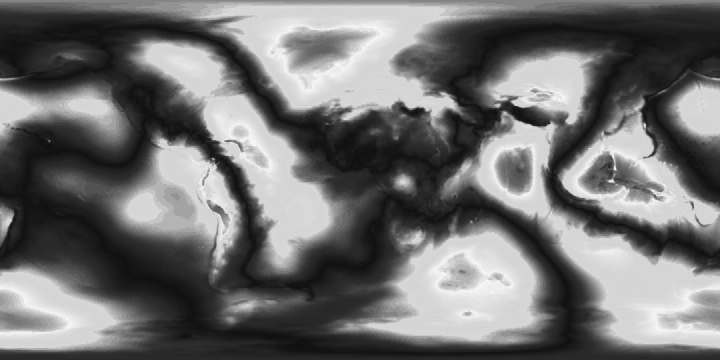
\includegraphics[width=\textwidth]{images/it_orig}
		  \caption{The EGM96 dataset evaluated on a spherical grid with uniformly distributed angles 
      $\paren{\vtheta_{l}}_{l=0}^{L-1}$, $\paren{\vphi_{j}}_{j=0}^{J-1}$ with $\vtheta_{l} := \frac{l\pi}{L-1}$
      and $\vphi_{j} := \frac{j 2\pi}{J}$ for $L = 360$ and $J = 720$. The horizontal axis 
      corresponds to the angles $\vphi_{j}$ whereas the vertical axis corresponds to the angles $\vtheta_{l}$.}
		  \label{Applications:egm96}
		\end{figure}    

    The corresponding function $f = \sum_{(k,n) \in \mathcal{I}^M} a_{k}^n Y_{k}^n$ was 
    evaluated on the Clenshaw-Curtis grid 
    $\mathcal{X}^{\cc}$ for $M = 360$, consisting of $2(M+1)(2M+1) = 520,562$
    nodes $\V{\xi}_{d}$. The CGNR algorithm was 
    applied with weight matrix $\V{W} := \V{W}^{\cc}$ containing the corresponding 
    quadrature weights. We used $\V{a}_{0} := \V{0}$ as initial guess. 
    The computation confirms the theoretical expectation that the algorithm already 
    terminates after one step, since the first iterate $\V{a}_{1}$ is computed as 
    $\V{a}_{1} = \V{Y} \: \V{W} = \V{Y}_{\mathcal{X}^{\cc}} \: \V{W}^{\cc} = \V{a}$.
    
    As a second test, we evaluated the function $f$ on a grid with nearly uniformly distributed
    nodes: We used a \emph{Healpix} grid with $D=786,432$ nodes. Healpix stands for 
    \emph{hierarchical equal area iso-latitude pixelization}. The corresponding grids 
    and accompanying software had been originally developed for applications in 
    cosmic microwave background experiments. The grid layout is described in  
    \begin{figure}[tb]
      \centering
      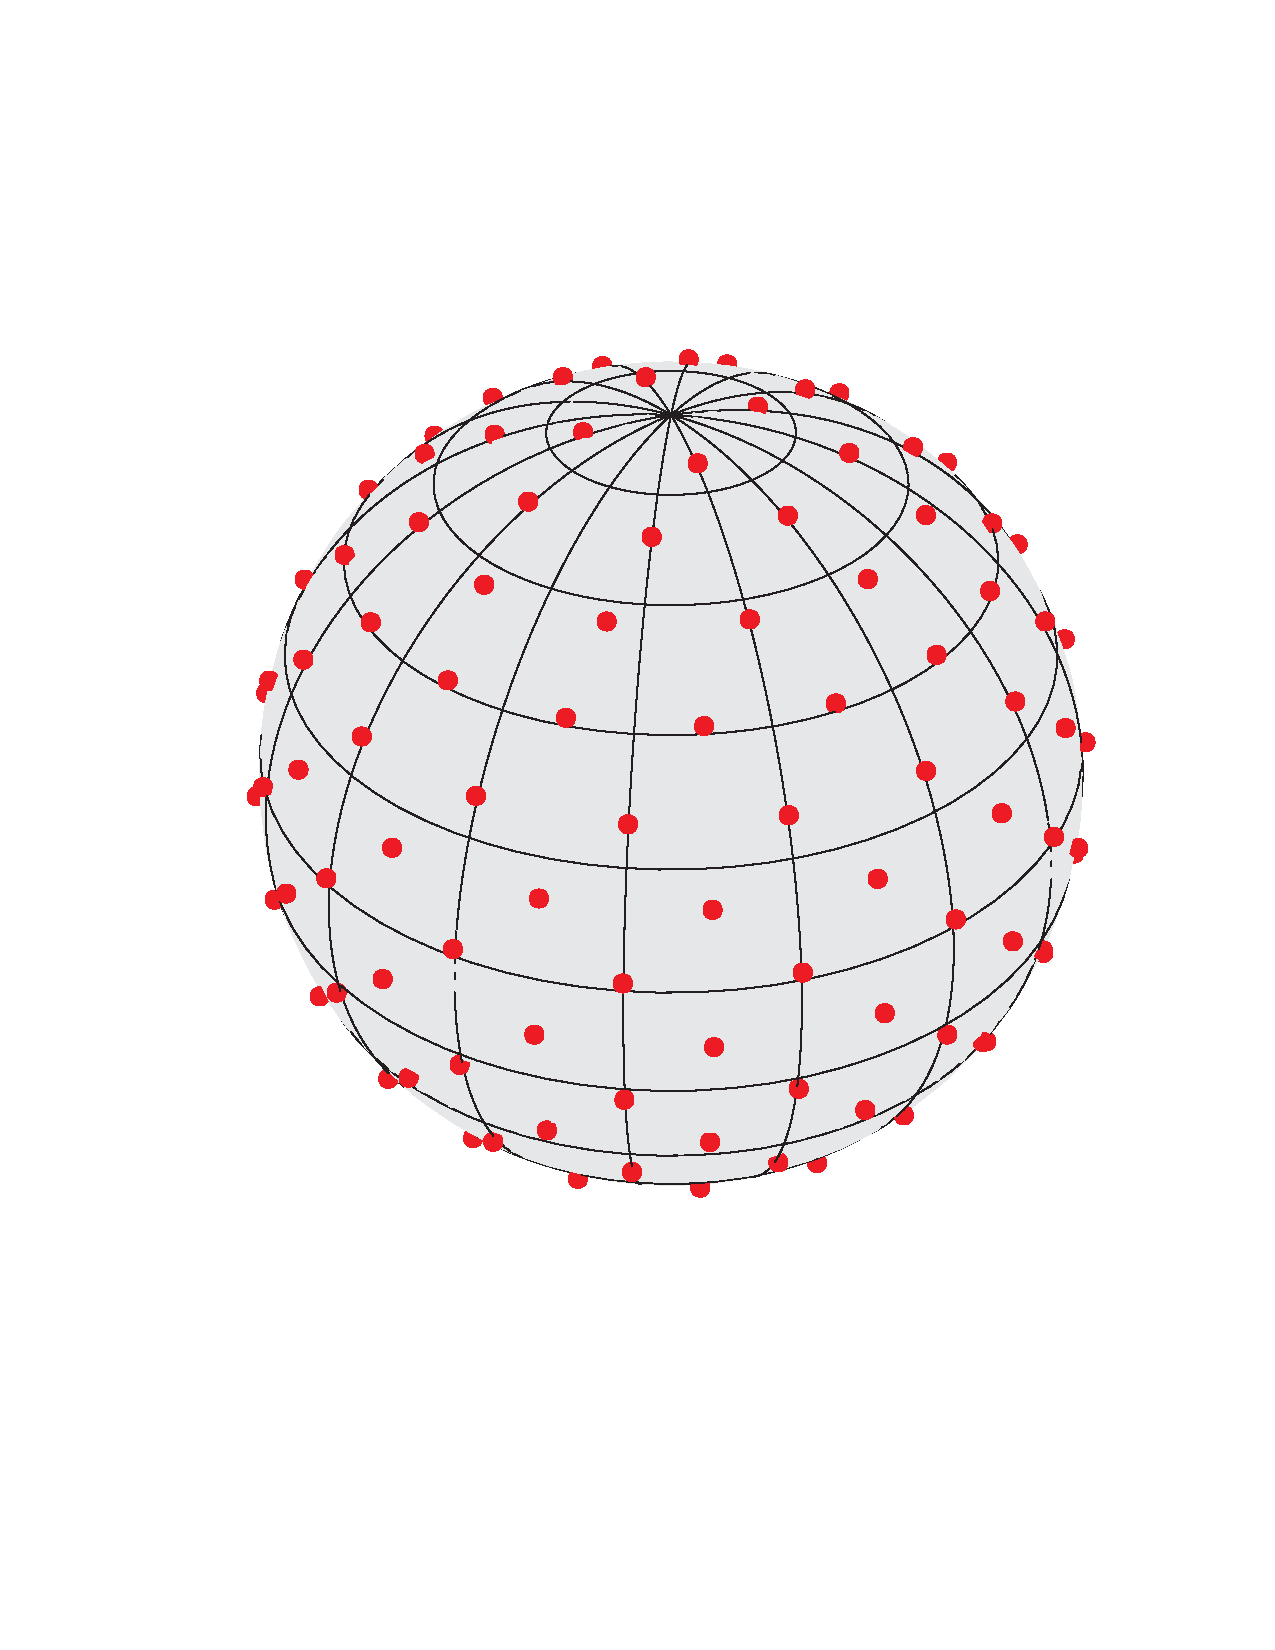
\includegraphics[width=0.6\textwidth]{images/healpix}
      \caption{A Healpix grid with $D = 192$ almost uniformly nodes.}
      \label{Applications:healpix}
    \end{figure}  
    \cite{healpix} and illustrated in Figure \ref{Applications:healpix}. The nodes are distributed 
    almost uniformely over the entire sphere $\twosphere$ which gives rise to choosing the weight matrix 
    $\V{W}$ for the CGNR algorithm to be the unity matrix, i.e. $\V{W} := \V{I}$. We used as 
    initial guess $\V{a}_{0} = \paren{a_{k,0}^n}_{(k,n) \in \mathcal{I}^M}$ with $a_{k,0}^n := 
    \frac{1}{\sqrt{2k+1}}$. Table \ref{tab:Healpix} shows the first $10$ iterations of the CGNR method which 
    converges after 6 iterations.    
    
		\begin{table}[ht]
		  \begin{center}
         \begin{tabular}{r|r|r}
         Iteration & $\norm{r}_{2}$ & $\norm{r_{l}}_{\infty}/\norm{f}_{\infty}$ \\[0.7ex] \hline
                 0 &    1.1913E+04 &        8.0377E+07 \\
                 1 &    3.5414E+01 &        2.1553E+06 \\
                 2 &    2.2627E-01 &        9.8485E+03 \\
                 3 &    6.2569E-04 &        2.0326E+01 \\
                 4 &    1.6942E-05 &        8.8598E-01 \\
                 5 &    9.6759E-08 &        4.5782E-03 \\
                 6 &    9.8756E-09 &        5.8426E-05 \\
                 7 &    9.8753E-09 &        5.8424E-05 \\
                 8 &    9.8753E-09 &        5.8424E-05 \\
                 9 &    9.8753E-09 &        5.8424E-05 \\
                10 &    9.8753E-09 &        5.8424E-05 \\
        \end{tabular}
		  \end{center}
		  \caption{Fourier reconstruction from EGM96 data evaluated on a healpix grid with $D=786,432$ nodes. 
		  For the first $10$ iterations, the 2-norm $\norm{\V{r}_{l}}_{2}$ of the residual $\V{r}_{l} := \V{f} - 
		  \V{Y}\:\V{a}_{l}$ and the relative residual error $\norm{r_{l}}_{\infty}/\norm{f}_{\infty}$ 
		  for the iterates $\V{a}_{l}$ in the CGNR method are shown. The method converges after $6$ iterations
		  yielding a final 2-norm of the residual $\norm{r_{6}} = 9.8753 \cdot 10^{-9}$.}
		  \label{tab:Healpix}
		\end{table}
		
  \end{example}
  
\subsection{The Weighted Optimal Interpolation Problem}
  For a comparatively high bandwidth, i.e. $(M+1)^2 > D$, the matrix $\V{Y}$ 
  has less rows than columns and the system \eqref{Applications:Problem} is 
  underdetermined. We therefore consider the following problem:
  \begin{definition}
    Let $M \in \NZ$, $D \in \N$, $\mathcal{X}=\paren{\V{\xi}_{d}}_{d=0}^{D-1} \subset \twosphere$, 
    $\V{f}=\paren{f_{d}}_{d=0}^{D-1} \in \C^{D}$ and 
    \[
      \V{\hat{W}} := \fun{\diag}{\paren{\hat{w}_{k}^n}_{(k,n) \in \mathcal{I}^M}},\quad 
      \hat{w}_{k}^n \in \Rp \ \paren{(k,n) \in \mathcal{I}^M}
    \]
    be given with $(M+1)^2 > D$. The problem of finding a vector $\V{a}=\paren{a_{k}^n}_{(k,n) 
    \in \mathcal{I}^M}$ of spherical Fourier coefficients with
    \begin{equation}
      \label{Applications:Min2}
      \norm{\V{a}}_{\V{hat{W}}}^2 = \text{min!, subject to } \V{Y}\:\V{a} = \V{f},
    \end{equation}
    is called a \emph{weighted optimal interpolation problem}.
  \end{definition}
  Since the linear system of equations \eqref{Applications:Problem} is underdetermined, we have the 
  additional possibility of choosing an 'optimal' interpolative vector of spherical Fourier coefficients 
  out of all vectors $\V{a}$ which meet the condition $\V{Y}\:\V{a} = \V{f}$. The optimal 
  interpolant is chosen to minimize a weighted euclidean norm $\norm{\cdot}_{\V{\hat{W}}}$. 
  Here, the idea of using a weighted norm is to impose smoothness conditions on the optimal interpolant. 
  Reasonable choices are often weights that correspond to Sobolev norms which also penalize the derivatives
  of the interpolative polynomial. The following lemma shows that a solution to
  \eqref{Applications:Min2} can be obtained as a solution of a 
  \emph{weighted normal equation of the second kind}.
  \begin{lemma}
    Problem \eqref{Applications:Min} is equivalent to the 
    \emph{weighted normal equation of the second kind}
    \begin{equation}
      \label{Applications:NormalEquation2}
      \V{Y} \: \V{\hat{W}}^{-1} \: \V{Y}^{\h} \V{z} = \V{f},\ \V{a} = \V{\hat{W}}^{-1}\:\V{Y}^{\h}\:\V{z}.
    \end{equation}
    Moreover, \eqref{Applications:NormalEquation1} has at least one solution.
    The solution is unique if the matrix $\V{Y}$ has full rank.
  \end{lemma}
  \begin{proof}
    We set $\V{b} := \V{\hat{W}}^{1/2}\:\V{a}$ and obtain from $\V{Y}\:\V{a} = \V{f}$ the equivalent 
    side condition $\V{Y}\:\V{\hat{W}}^{-1/2}\:\V{b} = \V{f}$. We have therefore
    \[
      \norm{\V{a}}_{\V{\hat{W}}}^2 = \norm{\V{\hat{W}}^{1/2}\:\V{a}}_{2}^2 = \norm{\V{b}}_{2}^2.
    \]
    The vector $\V{b}$ as minimizer of $\norm{\V{b}}_{2}^2$ under the side condition 
    $\V{Y}\:\V{\hat{W}}^{-1/2}\:\V{b} = \V{f}$ must fulfill $\V{b} \perp \fun{\mathcal{N}}{\V{Y}\:\V{\hat{W}}^{-1/2}}$ 
    which is equivalent to $\V{b} \in \fun{\mathcal{R}}{\V{\hat{W}}^{-1/2}\:\V{Y}^{\h}}$. Therefore, there exists a vector
    $\V{z}$ such that $\V{b} = \V{W}^{-1/2}\:\V{Y}^{\h}\: \V{z}$. Inserting this result into 
    $\V{Y}\:\V{\hat{W}}^{-1/2}\:\V{b} = \V{f}$, we find
    \begin{equation}
      \label{Applications:eq2}
      \V{Y} \: \V{\hat{W}}^{-1} \: \V{Y}^{\h} \V{z} = \V{f},\ \V{a} = \V{\hat{W}}^{-1}\:\V{Y}^{\h}\:\V{z}.
    \end{equation}
    Equation \eqref{Applications:eq2} has at least one solution since the matrix $\V{Y}\:\V{W}^{-1/2}\:\V{Y}^{\h}$
    is hermitian positive semi-definite. If the matrix $\V{Y}$ has full rank, the solution is unique 
    since the matrix $\V{Y}\:\V{W}^{-1/2}\:\V{Y}^{\h}$ is then even strictly hermitian positive definite
    and therefore non-singular.
  \end{proof}
  
  The CG method can also be modified for the weighted normal equation of the second kind. The corresponding 
  algorithm is denoted CGNE where 'E' now stands for 'error'. Further investigations on this problem where 
  behind the scope of this text and not considered, but are interesting for future applications of the 
  presented algorithms. We therefore close our investigations on iterative Fourier reconstruction with the 
  remark that this section only provided a small glance at this relatively new technique.
